\documentclass[tikz]{standalone}
\usetikzlibrary{matrix}
\usetikzlibrary{calc}
\usepackage{tikz-3dplot}
\usepackage{amsmath}
\usepackage{amsthm}
\usepackage{amssymb}

\newcommand{\ba}{\mathbf{a}}

\begin{document}
%%%%%%%%%%%
%
% BASIS OF R^2
%
%%%%%%%%%%%
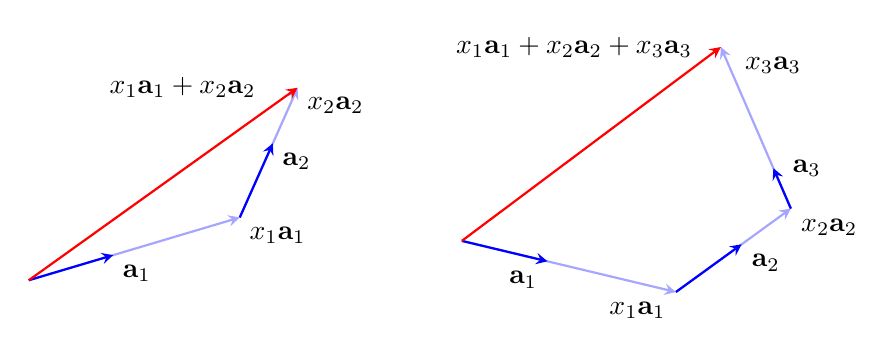
\begin{tikzpicture}[
vector/.style={-stealth, thick}
]

\begin{scope}[shift={(-5.5,-0.5)}, rotate=-10]
\def\Px{1}
\def\Py{0.5}
\def\Qx{0.25}
\def\Qy{1}

\def\a{2.5}
\def\b{1.75}
\def\u{0.8}

\coordinate (O) at (0, 0);
\coordinate (P) at (\Px, \Py);
\coordinate (Q) at (\Qx, \Qy);
\coordinate (aP) at (\a*\Px, \a*\Py);
\coordinate (aPplusQ) at (\a*\Px + \Qx, \a*\Py + \Qy);
\coordinate (bQ) at (\b*\Qx, \b*\Qy);

\coordinate (R) at (\a*\Px + \b*\Qx, \a*\Py + \b*\Qy);
\coordinate (RR) at (\u*\a*\Px + \u*\b*\Qx, \u*\a*\Py + \u*\b*\Qy);


\node[below right] at (P) {$\ba_1$};
\node[below right] at (aPplusQ) {$\ba_2$};


\node[below right] at (aP) {$x_1\ba_1$};
\node[below right] at (R) {$x_2\ba_2$};
\node[left] at (R) {$x_1\ba_1 + x_2\ba_2\quad\,$};


\draw[vector, thick, blue!35] (O) -- (aP);
\draw[vector, thick, blue!35] (aP) -- (R);

\draw[vector, blue] (O) -- (P);
\draw[vector, blue] (aP) -- (aPplusQ);
\draw[vector, red] (O) -- (R);
\end{scope}

\begin{scope}[rotate=-40]
\def\Px{1}
\def\Py{0.5}
\def\Qx{0.25}
\def\Qy{1}
\def\Rx{-0.5}
\def\Ry{0.25}

\def\a{2.5}
\def\b{1.75}
\def\c{4}

\coordinate (O) at (0, 0);
\coordinate (P) at (\Px, \Py);
\coordinate (aP) at (\a*\Px, \a*\Py);
\coordinate (aPplusQ) at (\a*\Px + \Qx, \a*\Py + \Qy);
\coordinate (aPplusbQ) at (\a*\Px + \b*\Qx, \a*\Py + \b*\Qy);
\coordinate (aPplusbQplusR) at (\a*\Px + \b*\Qx + \Rx, \a*\Py + \b*\Qy + \Ry);
\coordinate (aPplusbQpluscR) at (\a*\Px + \b*\Qx + \c*\Rx, \a*\Py + \b*\Qy + \c*\Ry);




\draw[vector, thick, blue!35] (O) -- (aP) node [below left, black] {$x_1\ba_1$};
\draw[vector, thick, blue] (O) -- (P) node [below left, black] {$\ba_1$};

\draw[vector, thick, blue!35] (aP) -- (aPplusbQ) node [below right, black] {$x_2\ba_2$};
\draw[vector, thick, blue] (aP) -- (aPplusQ) node [below right, black] {$\ba_2$};
;

\draw[vector, thick, blue!35] (aPplusbQ) -- (aPplusbQpluscR) node [below right, black] {$\,\,\,x_3\ba_3$};
\draw[vector, thick, blue] (aPplusbQ) -- (aPplusbQplusR) node [right, black] {$\,\,\ba_3$}; 

\draw[vector, red] (O) -- (aPplusbQpluscR) node[left, black] {$x_1\ba_1 + x_2\ba_2 + x_3\ba_3\,\,\,\,$};

\end{scope}
\end{tikzpicture}

\end{document}
